\subsection{UMTS (3G)}
\selectlanguage{russian}

В третьем поколении мобильных сетей, называемом UMTS, защищённость немного улучшена. Общая схема аутентификации (рис.~\ref{fig:gsm3}) осталась примерно такой же, как и в GSM. Жирным шрифтом на рисунке выделены новые добавленные элементы по сравнению с GSM.
\begin{enumerate}
    \item Производится взаимная аутентификация SIM-карты и центра аутентификации по токенам $\textrm{RES}$ и $\MAC$.
    \item Добавлены проверка целостности и аутентификация данных (имитовставка\index{имитовставка}).
    \item Используются новые алгоритмы создания ключей, шифрования и имитовставки\index{имитовставка}.
    \item Добавлены счётчики на SIM-карте $\textrm{SQN}_{\textrm{T}}$ и в центре аутентификации $\textrm{SQN}_{\textrm{Ц}}$ для защиты от атак воспроизведения. Значения увеличиваются при каждой попытке аутентификации и должны примерно совпадать.
    \item Увеличена длина ключа шифрования до 128 бит.
\end{enumerate}

\begin{figure}[!ht]
	\centering
	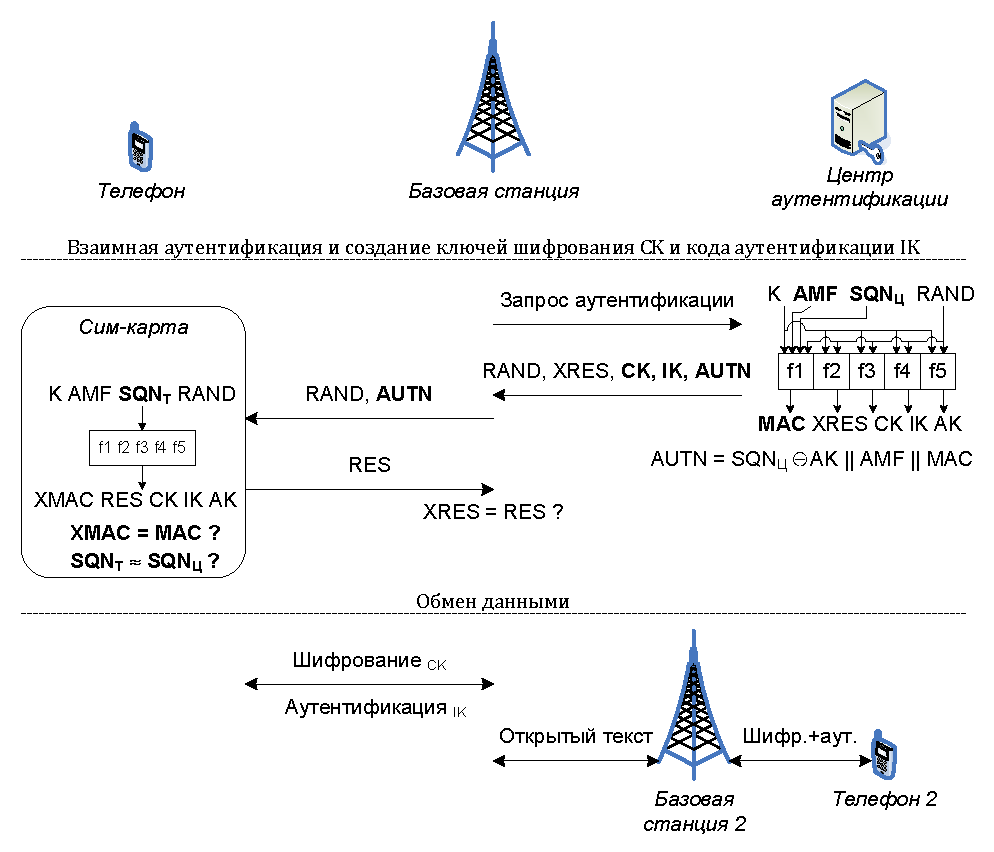
\includegraphics[width=\textwidth]{pic/gsm3}
	\caption{Взаимная аутентификация и шифрование в UMTS (3G)\label{fig:gsm3}}
\end{figure}

Обозначения на рис.~\ref{fig:gsm3} следующие:
\begin{itemize}
    \item K -- общий секретный 128-битовый ключ SIM-карты и центра аутентификации;
    \item RAND -- 128-битовое псевдослучайное число, создаваемое центром аутентификации;
    \item $\textrm{SQN}_{\textrm{T}}$, $\textrm{SQN}_{\textrm{Ц}}$ -- 48-битовые счётчики для защиты от атак воспроизведения;
    \item AMF -- 16-битовое значение окна для проверки синхронизации счётчиков;
    \item CK, IK, AK -- 128-битовые ключи шифрования данных CK, кода аутентификации данных IK, гаммы значения счётчика AK;
    \item MAC, XMAC -- 128-битовые аутентификаторы центра SIM-карте;
    \item RES, XRES -- 128-битовые аутентификаторы SIM-карты центру;
    \item AUTN -- вектор аутентификации.
\end{itemize}

Алгоритмы $fi$ не фиксированы стандартом и выбираются при реализациях.

Из оставшихся недостатков защиты персональных данных можно перечислить.
\begin{enumerate}
    \item Уникальный идентификатор SIM-карты IMSI (\langen{International Mobile Subscriber Identity}) по-прежнему передаётся в открытом виде, что позволяет злоумышленнику идентифицировать абонентов по началу сеанса регистрации SIM-карты в мобильной сети.
    \item Шифрование и аутентификация производятся только между телефоном и базовой станцией, а не между двумя телефонами. Это является необходимым условием для подключения СОРМ (Система технических средств для обеспечения функций оперативно-розыскных мероприятий) по закону <<О связи>>. С другой стороны, это повышает риск нарушения конфиденциальности персональных данных.
    \item Алгоритм шифрования A5/3\index{шифр!A5/3} (KASUMI)\index{шифр!KASUMI} на 128-би\-то\-вом ключе теоретически взламывается атакой на связанных ключах основе известного открытого текста для 64 MB данных с использованием 1 GiB памяти за $2^{32}$ операций (2 часа на обычном ПК 2010 года,~\cite{Dunkelman:Keller:Shamir:2010}).
\end{enumerate}
